En esta sección, vamos a realizar experimentos para comprobar empíricamente tanto el tiempo de ejecución como la calidad de las soluciones devueltas por nuestro algoritmo goloso.

Como ya sabemos, el algoritmo de Dijkstra devuelve el camino de un nodo inicial hacia todos. Particularmente, a nosotros nos interesa el camino de $u$ a $v$. Por esto, se nos ocurrió una simple optimización: cortar la ejecución del algoritmo cuando alcanza $v$.

\begin{figure}[H]
  \begin{minipage}{0.5\linewidth}
    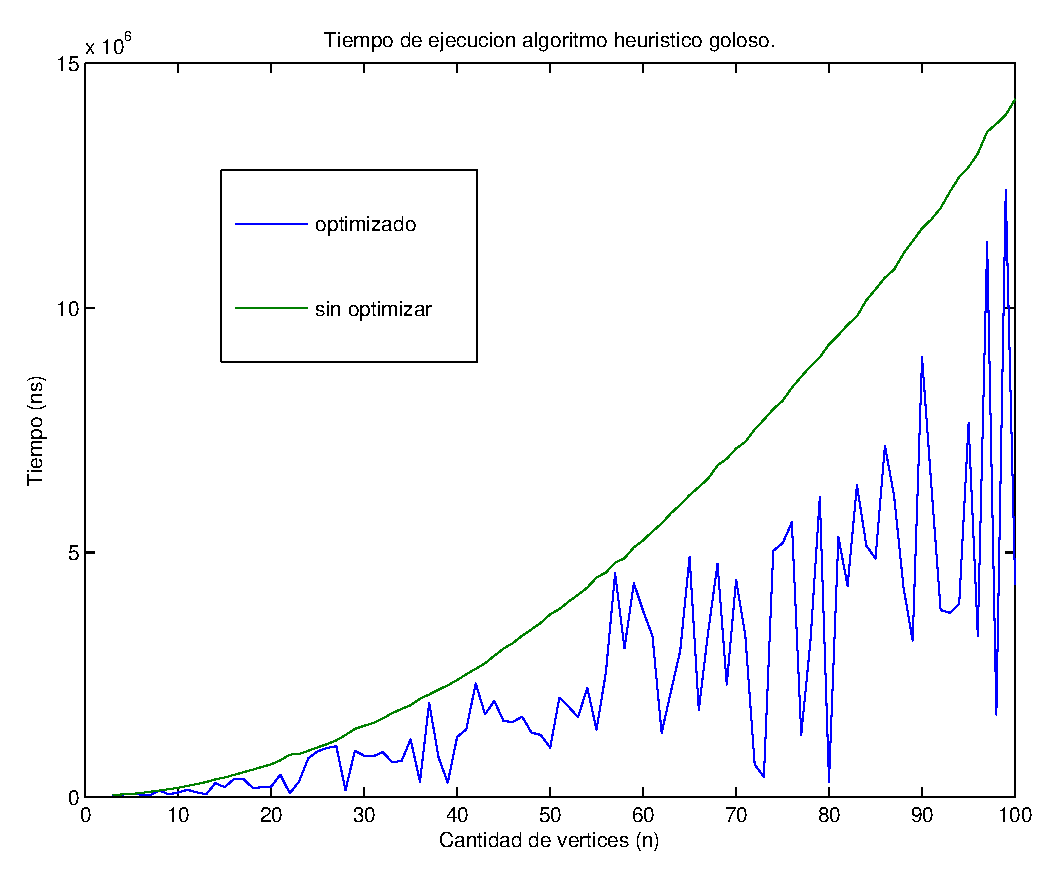
\includegraphics[width=\linewidth]{graficos/goloso_tiempo.eps}
    \caption{Tiempo ejecución goloso}\label{fig:goloso-tiempo}
  \end{minipage}
  \hfill
  \begin{minipage}{0.5\linewidth}
    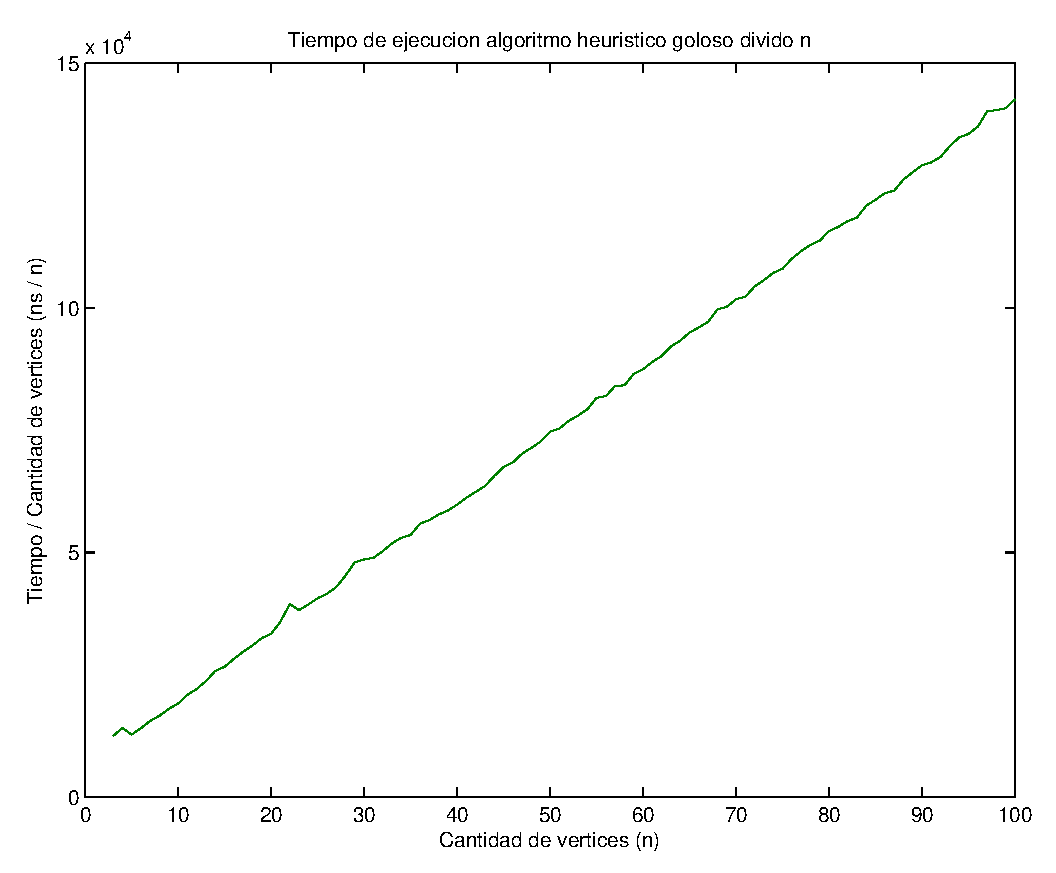
\includegraphics[width=\linewidth]{graficos/goloso_tiempo_div_n.eps}
    \caption{Goloso sin optimización}\label{fig:goloso-tiempo-n}
  \end{minipage}
\end{figure}

Como se puede observar tanto en la Figura \ref{fig:goloso-tiempo} como en la Figura \ref{fig:goloso-tiempo-n}, nuestro algoritmo sin la optimización se comporta de forma cuadrática. Esto es lógico ya que nuestro algoritmo sin la optimización corre el algoritmo de Dijkstra de principio a fin, utilizando listas de adyacencia.

Además, en la figura \ref{fig:goloso-tiempo} podemos observar que el algoritmo con la optimización tiene un tiempo de ejecución menor o igual al algoritmo sin la optimización. Esto depende del momento en que el algoritmo de Dijkstra encuentra a $v$.

Luego, nos propusimos comparar la calidad de las soluciones entre el goloso y el exacto, para casos aleatorios. Cabe aclarar que vamos a utilizar casos con valores bajos de $n$, ya que el algoritmo exacto tiene tiempo de ejecución exponencial.

\begin{center}
 \begin{tabular}{|c|c|}
      \hline
      n&error proporcional \\
      \hline
      3&1\\
      4&1.00029\\
      5&1.0015\\
      6&1.00219\\
      7&1.00233\\
      8&1.00285\\
      9&1.00252\\
      10&1.0022\\
      \hline
    \end{tabular}
\end{center}

Como se puede observar en la tabla de arriba, el error proporcional del algoritmo goloso respecto del algoritmo exacto para grafos con pocos nodos, es muy pequeño. Por esta razón, no vamos a incluir gráficos que comparen dichos algoritmos, ya que es difícil de apreciar visualmente.


% \begin{figure}[H]
%   \begin{minipage}{0.25\linewidth}
%     \begin{tabular}{|c|c|}
%       \hline
%       n&error proporcional \\
%       \hline
%       3&1\\
%       4&1.00029\\
%       5&1.0015\\
%       6&1.00219\\
%       7&1.00233\\
%       8&1.00285\\
%       9&1.00252\\
%       10&1.0022\\
%       \hline
%     \end{tabular}
%   \end{minipage}
%   \begin{minipage}{0.25\linewidth}
%     \begin{tabular}{|c|c|}
%       \hline
%       n&error proporcional \\
%       \hline
%       3&1\\
%       4&1.00029\\
%       5&1.0015\\
%       6&1.00219\\
%       7&1.00233\\
%       8&1.00285\\
%       9&1.00252\\
%       10&1.0022\\
%       \hline
%     \end{tabular}
%   \end{minipage}
%     \begin{minipage}{0.25\linewidth}
%     \begin{tabular}{|c|c|}
%       \hline
%       n&error proporcional \\
%       \hline
%       3&1\\
%       4&1.00113\\
%       5&1.00189\\
%       6&1.00521\\
%       7&1.00588\\
%       8&1.00966\\
%       9&1.013\\
%       10&1.01641\\
%       \hline
%     \end{tabular}
%   \end{minipage}
%     \begin{minipage}{0.25\linewidth}
%     \begin{tabular}{|c|c|}
%       \hline
%       n&error proporcional \\
%       \hline
%       3&1\\
%       4&1\\
%       5&1\\
%       6&1\\
%       7&1.00001\\
%       8&1.00103\\
%       9&1.00329\\
%       10&1.00442\\
%       \hline
%     \end{tabular}
%   \end{minipage}
% \end{figure}

En los siguientes gráficos, vamos a comparar empíricamente la proporción entre los pesos $\omega_2$ totales entre las soluciones del algoritmo exacto y el goloso para la familia de grafos previamente mencionada. Creamos una función, la cual recibe un parámetro que es la diferencia deseada entre el goloso y el exacto. Recordemos que dijimos que podemos hacer que la diferencia entre la solución óptima y la que devuelve nuestro algoritmo goloso para esta familia puede ser tan grande como queramos.

Sea $S$ la solución devuelta por el algoritmo exacto, y $S'$ la solución devuelta por el algoritmo goloso, vamos a graficar $\omega_2(S')$ / $\omega_2(S)$ para distintos $n$.

\begin{figure}[H]
  \begin{minipage}{0.5\linewidth}
    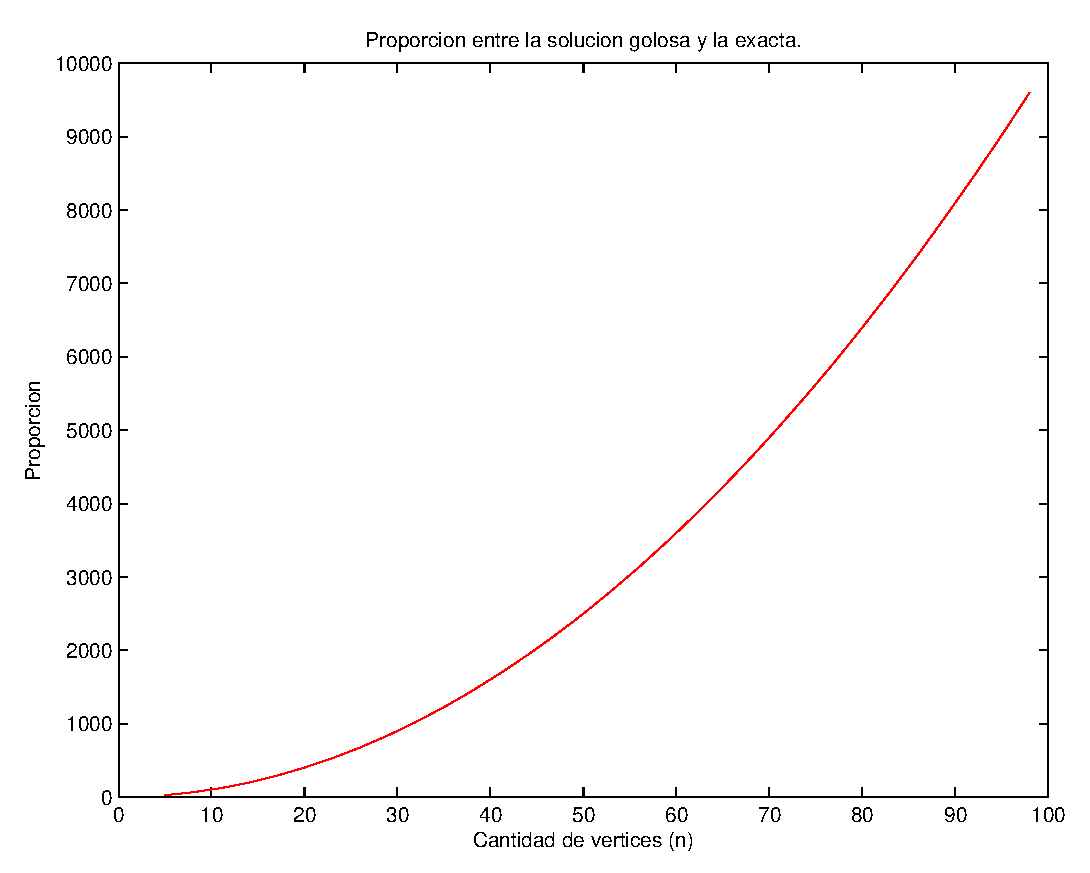
\includegraphics[width=\linewidth]{graficos/goloso_proporcion.eps}
    \caption{Comparación goloso exacto función $n^2$}\label{fig:goloso-n2}
  \end{minipage}
  \hfill
  \begin{minipage}{0.5\linewidth}
    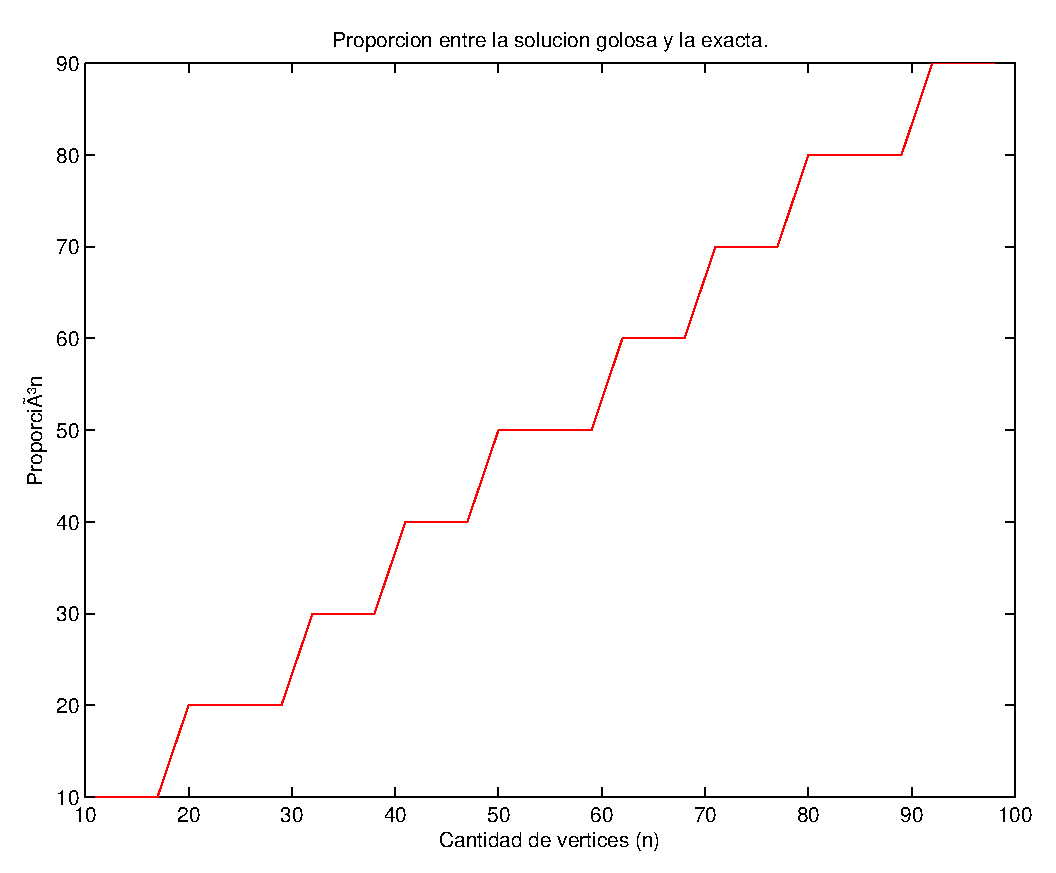
\includegraphics[width=\linewidth]{graficos/goloso_proporcion2.eps}
    \caption{Comparación goloso exacto escalonado}\label{fig:goloso-escalonado}
  \end{minipage}
\end{figure}

En el gráfico \ref{fig:goloso-n2} colocamos la diferencia de $n^2$ para cada $n$, mientras que en el gráfico \ref{fig:goloso-escalonado} utilizamos la siguiente función:
\begin{verbatim}
error(n) = n - (n mod 10)
\end{verbatim}

Cabe aclarar que estos gráficos utilizan valores de $n$ mayores a 10, ya que el error tiene que ser mayor o igual a uno. En el caso en que se use un error menor a 1, el algoritmo no funciona ya que esto significaría que es ``más exacto'' que el exacto.

De esta forma, podemos asegurar que nuestro algoritmo goloso no es $\alpha$-aproximado para esta familia de grafos. Esto se puede observar fácilmente, ya que dado un $\alpha$ podemos generar un grafo donde el error proporcional sea mayor a $\alpha$.